\documentclass[11pt]{article}

% Camera-ready submission build.
\usepackage[final]{acl}
\usepackage{dblfloatfix}
\usepackage{times}
\usepackage{latexsym}
\usepackage[T1]{fontenc}
\usepackage[utf8]{inputenc}
\usepackage[british]{babel}
\usepackage{microtype}
\usepackage{graphicx}
\usepackage{float}
\usepackage{placeins}
\usepackage{booktabs}

\title{Neural Authorship Attribution with Subword Embeddings and CNN-LSTM}

\author{Mekhail Muller (u21632792) \And Ruan Nel (u25748956) \And Mosa Phalane (u14168970) \\
  \textbf{Group 38}, COS760, University of Pretoria}

\begin{document}
\maketitle

\begin{abstract}
We investigate authorship attribution on social media microtext using BPE subword tokenisation combined with a CNN-LSTM architecture. The model learns author-specific stylometric fingerprints from subword sequences and classifies tweets to their authors. We compare against eight baselines (BoW, TF-IDF, character $n$-grams, word $n$-grams, each with SVM and logistic regression) under identical stratified splits on a 50-author Twitter corpus. The CNN-LSTM ensemble achieves 63.8\% accuracy and 0.640 macro-F$_1$, while the best baseline (character $n$-grams + SVM) reaches 66.2\% accuracy and 0.657 macro-F$_1$. SHAP and LIME analyses reveal the model relies on morphological fragments, punctuation habits, and author-specific abbreviations. Error analysis shows misclassifications concentrate among authors sharing topical vocabulary and short post lengths.
\end{abstract}

\section{Problem Statement}
\label{sec:problem}

Authorship attribution on short social text remains difficult because posts are noisy, vocabulary-overlapping, and sparse per author. We ask: \textbf{(RQ1)} Can a subword-based CNN-LSTM learn stable authorship representations from microtext? \textbf{(RQ2)} How does it compare to classical stylometric features under a fair, shared evaluation protocol? \textbf{(RQ3)} Which subword patterns and author pairs drive correct decisions and systematic confusion?

\section{Introduction}
\label{sec:intro}

Authorship attribution identifies who wrote a given text, with applications in forensic linguistics and social media analysis \citep{theophilo2021authorship}. Classical methods use bag-of-words, TF-IDF, and $n$-gram features but may miss sub-lexical writing habits \citep{suman2021authorship,modupe2022applied}. Subword tokenisation (BPE, WordPiece) decomposes text into morphemic units, handling rare forms compositionally \citep{sennrich2016neural}, yet its advantage over classical baselines for author discrimination on short text remains unclear.

We train a CNN-LSTM on BPE sequences and compare it against eight sparse-feature pipelines under identical conditions, integrating SHAP/LIME to interpret decisions. The remainder of this report covers related work (\S\ref{sec:related}), methodology (\S\ref{sec:method}), experiments (\S\ref{sec:experiments}), explainability (\S\ref{sec:explainability}), and conclusions (\S\ref{sec:conclusion}).

\section{Literature Survey}
\label{sec:related}

Authorship attribution has traditionally relied on sparse, frequency-based feature families: BoW, TF-IDF, and word/character $n$-grams, to capture an author's stylometric fingerprint \citep{theophilo2021authorship}. While effective for long-form text, these methods encounter sparsity and OOV issues on short social posts. Recent work emphasises dense representations via subword tokenisation (BPE, WordPiece), which decomposes text into morphemic units and surfaces sub-lexical patterns missed by word-level methods \citep{sennrich2016neural,hossain2025authornet}.

Contemporary systems such as AuthorNet \citep{hossain2025authornet} leverage transformer ensembles but are computationally heavy with limited transparency. Studies on microtext attribution \citep{suman2021authorship,modupe2022subword} employ deep models yet rarely isolate the interaction of subword embeddings with a hybrid CNN-LSTM for stylistic discrimination. \citet{modupe2022applied} apply regularised deep networks to post-authorship without systematic baseline comparison. Much subword-oriented research \citep{toraman2023tokenization,drzik2026morphology} targets general semantic tasks rather than individual writing styles.

\textbf{Gap:} A fair, head-to-head comparison between subword neural encoders and the full classical stylometric grid (4 feature families $\times$ 2 classifiers) under identical splits, combined with post-hoc SHAP/LIME explainability, remains unaddressed. We fill this gap.

\section{Approach, Methodology, and Data}
\label{sec:method}

\subsection{Dataset}
\label{sec:dataset}

We conduct \emph{closed-set} authorship attribution on \emph{Twitter-style microtext} from the public benchmark of \citet{suman2021authorship}, alongside related social-media attribution work~\citep{theophilo2021authorship} and deep stylometric models for short posts~\citep{modupe2022post}.
The release is \textbf{English} and mixed (news-style blurbs, @-replies, informal prose).
Messages are short and noisy (URLs, truncation in the export, hashtags, orthographic variation), which inflates \textbf{OOV} pressure, limits context per class, and allows \textbf{stylistic overlap} between authors~\citep{suman2021authorship}.

We default to the \textbf{200-messages-per-author} slice over the companion 50-per-author file because more text per writer stabilises parameter-heavy models (neural encoder and subword vocab) while keeping the same 50-author closed set; smaller slices remain available for ablations.

\emph{Experimental framing.} Closed-set attribution means every training / validation / test label is drawn from same fixed author catalogue \(C\); there is no held-out unseen writer at inference.\footnote{A practical limitation remains \emph{domain lock-in}: results do not transfer to long-form prose, different platforms, or languages without retraining.}

\paragraph{Provenance and availability.}
The raw tables are released with~\citet{suman2021authorship} in the public \href{https://github.com/chanchalIITP/AuthorIdentification}{AuthorIdentification GitHub repository}.
If missing locally, \texttt{python -m experiments.run\_cnn\_lstm --fetch-dataset} shallow-clones into \path{data/AuthorIdentification/}; \path{data/fetch_dataset.py} is an alternative fetch entry point.
We use the \path{200_tweets_per_user.csv} slice (default \texttt{DEFAULT\_CHANCHAL\_200\_CSV}); statistics and splits are in Table~\ref{tab:dataset-stats}.

\begin{table}[H]
  \centering
  \small
  \setlength{\tabcolsep}{3pt}
  \begin{tabular}{@{}p{0.58\columnwidth}r@{}}
    \hline
    \textbf{Statistic} & \textbf{Value} \\
    \hline
    Authors \(C\) & 50 \\
    Messages / author & 200 (balanced) \\
    Total labelled messages & 10{,}000 \\
    Train / val / test (seed 42) & 6{,}999 / 1{,}500 / 1{,}501 \\
    Authors in train / val / test & 50 / 50 / 50 \\
    Tokens: mean / med.\ / max & 13.3 / 13 / 33 \\
    Characters: mean / med.\ / max & 73.7 / 70 / 140 \\
    \hline
  \end{tabular}
  \caption{Chanchal \texttt{200\_tweets\_per\_user} slice: cleaned lengths and splits.}
  \label{tab:dataset-stats}
\end{table}

\paragraph{Schema and labels.}
The export we use stores \textbf{two unnamed columns} interpreted as \emph{text} then \emph{author} (header cells \texttt{0} / \texttt{1}); the shared \texttt{DatasetLoader} also accepts explicit \texttt{Text} / \texttt{Author} headers when present.

Author cells contain \textbf{numeric string identifiers} (Twitter user IDs), not human-readable display names; strings are sorted lexicographically and mapped bijectively to dense class indices \(0\ldots C{-}1\) for stable training across runs.

\paragraph{Illustrative instance (anonymised).}
\textit{``India and Benin should broaden trade ties: Tharoor - India and Benin need to broaden and deepen trade ties and look\ldots''} (one preprocessed row from \path{200_tweets_per_user.csv}; author ID omitted).

\paragraph{Train / validation / test split.}
Stratified partitioning uses two nested \texttt{StratifiedShuffleSplit} calls in \texttt{DatasetLoader.split} (scikit-learn) at \textbf{70\%/15\%/15\%}.
The split uses one random state (default \texttt{42}, overridable with \texttt{--split-seed} in the driver so it can differ from CNN weight initialisation seeds).
\textbf{All 10{,}000} cleaned rows enter the split on this CSV (no \emph{empty-string} drops in the default run); sizes \textbf{6{,}999 / 1{,}500 / 1{,}501} come from \textbf{stratified split rounding}, not row deletion.

All \textbf{fifty authors appear in train, validation, \emph{and} test} at non-zero count.

\textbf{Reporting conventions.} Validation \textbf{macro-F$_1$} drives early stopping; headline tables report \textbf{held-out test} macro and per-class summaries. Optional \texttt{--ensemble-train-seeds} retrains several CNN initialisations on the same split and aggregates test predictions by majority vote.

\subsection{Preprocessing}
\label{sec:preprocessing}
\texttt{Preprocessor} (\texttt{src/preprocessing.py}) applies a deterministic chain before splitting or vectorisation: HTTP(S) and \texttt{www.} URLs and \texttt{@}mentions are stripped; repeated whitespace is collapsed and trimmed.
\texttt{preserve\_punctuation=True} by default so punctuation stays in the string for stylometry; setting \texttt{False} removes non-alphanumeric symbols via a regex mask.
\texttt{.clean()} can return an empty string (e.g.\ URL-only posts); those rows are dropped before stratified splitting (\emph{none} on the default 200$\times$50 export).

\subsection{Subword Tokenisation}
\label{sec:tokenisation}

We train a BPE tokeniser (HuggingFace \texttt{tokenizers}, \texttt{src/tokeniser.py}) on the \textbf{training split only}, with default vocabulary size \(10^4\) (overridable via \texttt{--vocab-size}) and punctuation-isolation pre-tokenisation unless \texttt{--no-isolate-punctuation} is set.
Sequences are padded/truncated to \texttt{max\_seq\_len}=384.
This captures morphological fragments (prefixes, suffixes, misspellings) as author-specific cues and eliminates OOV issues since any text decomposes into known subwords \citep{sennrich2016neural}.

\subsection{Neural Model: CNN-LSTM}
\label{sec:cnn-lstm}
\texttt{CNNLSTMModel} (\texttt{src/model.py}) maps token IDs through an embedding layer with dropout, then \textbf{parallel \texttt{Conv1d}} branches with kernel sizes \([2,3,4]\) and ReLU.
Each branch yields a length-\(T-k+1\) feature map; maps are \textbf{right-padded to length \(T\)} and concatenated along the channel axis (\(3\times256\) filters in the default driver), with dropout applied on the CNN stack.
The resulting \([B,T,F\cdot K]\) tensor is processed by a \textbf{stacked LSTM} (two layers in the driver configuration) \textbf{along the time dimension}.
A \textbf{global max-over-time} readout on LSTM outputs forms the document vector, which passes through dropout into a linear layer producing \(C\) class logits.

\subsection{Baseline Feature Extractors and Classifiers}
\label{sec:baselines}

\paragraph{Feature extractors.}
\texttt{BaselineFeatureExtractor} (\texttt{src/features.py}) materialises four sparse views on the same cleaned splits: \textbf{BoW} (word unigram counts), \textbf{TF-IDF} (word unigrams), \textbf{character $n$-grams} (TF-IDF on character 3--5-grams with \texttt{char\_wb} analyser), and \textbf{word $n$-grams} (TF-IDF on unigrams and bigrams).
Vectorisers use scikit-learn defaults with lowercasing; vocabulary is capped at 10{,}000 features per extractor.

\paragraph{Classifiers.}
Each feature matrix feeds \textbf{linear SVM} (\texttt{LinearSVC}, $C{=}1.0$) and \textbf{multinomial logistic regression} ($C{=}1.0$, \texttt{max\_iter}${=}1000$) via \texttt{src/sparse\_baselines.py}.
All eight (feature $\times$ classifier) pairs are evaluated on the identical stratified split (seed 42); metrics are aggregated in \texttt{results/metrics.json}.

\subsection{Training protocol}
\label{sec:hparams}
\texttt{Trainer} (\texttt{src/trainer.py}) uses the Adam optimiser with gradient clipping (\texttt{max\_norm}=1.0), tracks validation macro-\(F_1\) each epoch, checkpoints the best validation weights, and stops when macro-\(F_1\) fails to improve for \texttt{patience} epochs (bounded by \texttt{epochs}).
On CUDA, training normally uses automatic mixed precision (disable with \texttt{--no-amp}) and may use fused Adam when supported (\texttt{--no-fused-adam} disables).
Repository defaults: learning rate \(8{\times}10^{-4}\), weight decay \(10^{-4}\), label smoothing \(0.02\), dropout \(0.30\), embedding dimension \(256\), \(256\) filters per kernel width, LSTM hidden \(384\) (two layers), vocabulary \(10^4\), max sequence \(384\), inverse-frequency loss weights, up to \(100\) epochs (patience \(24\)), and \texttt{ReduceLROnPlateau}; batch size is auto-sized via \texttt{training\_hardware.py} when omitted.

\paragraph{Optional pretrained embeddings (experimental).}
By default the embedding table is trained from scratch on BPE ids.
The driver also supports optional \textbf{transfer-style initialisation} from an external FastText \texttt{.vec} file (\texttt{src/pretrained\_embeddings.py}) via the \texttt{--fasttext-vec}, \texttt{--fasttext-limit}, and \texttt{--freeze-pretrained} flags; this path is experimental and our \textbf{reported ensemble did not use it} (random init + train-fit BPE only).
Runs write checkpoints and logs under timestamped \path{artifacts/runs/}.

\begin{figure*}[!t]
  \centering
  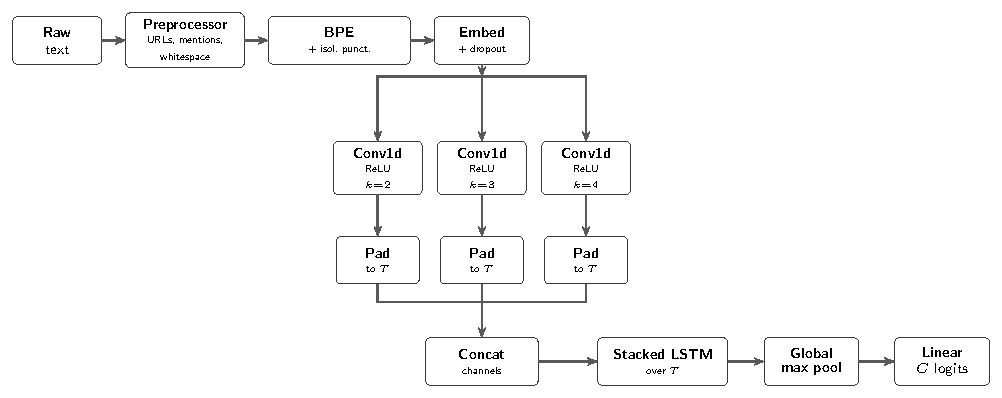
\includegraphics[width=\textwidth]{figures/pipeline.pdf}
  \caption{Neural attribution pipeline (cf.\ \texttt{Preprocessor}, \texttt{SubwordTokeniser}, \texttt{CNNLSTMModel}): raw text \(\rightarrow\) clean \(\rightarrow\) BPE with punctuation-isolation pre-tokenisation \(\rightarrow\) embedding \(\rightarrow\) parallel Conv1d branches (ReLU; pad each map to length \(T\), concat channels) \(\rightarrow\) stacked LSTM over \(T\) \(\rightarrow\) global max-over-time \(\rightarrow\) linear logits over \(C\) authors.}
  \label{fig:pipeline}
\end{figure*}

\section{Experiments and Results}
\label{sec:experiments}

\subsection{Experimental Setup}

All experiments use the Chanchal 200$\times$50 slice with stratified 70/15/15 splits (seed 42).
Neural training runs on CUDA (Windows 11, NVIDIA RTX 5090); sparse baselines run on CPU in the same driver invocation (\texttt{python -m experiments.run\_cnn\_lstm --fetch-dataset}).
Headline numbers below are read from \texttt{results/metrics.json} (schema version 2).

\subsection{Overall Comparison}

Table~\ref{tab:main-results} summarises held-out \textbf{test} accuracy and macro-F$_1$ for the CNN-LSTM ensemble (seeds 42, 5, 98; majority vote) and all eight sparse baselines.

\begin{table*}[!bt]
  \centering
  \footnotesize
  \setlength{\tabcolsep}{4pt}
  \begin{tabular}{lcccc}
    \hline
    \textbf{System} & \textbf{Acc.} & \textbf{P$_{\mathrm{macro}}$} & \textbf{R$_{\mathrm{macro}}$} & \textbf{$F_{1,\mathrm{macro}}$} \\
    \hline
    Char.\ $n$-gram + SVM & 0.662 & 0.658 & 0.662 & \textbf{0.657} \\
    CNN-LSTM ensemble & 0.638 & 0.651 & 0.638 & 0.640 \\
    Char.\ $n$-gram + LR & 0.634 & 0.633 & 0.634 & 0.626 \\
    TF-IDF + SVM & 0.586 & 0.583 & 0.586 & 0.582 \\
    Word $n$-gram + SVM & 0.577 & 0.573 & 0.577 & 0.570 \\
    TF-IDF + LR & 0.567 & 0.566 & 0.567 & 0.560 \\
    Word $n$-gram + LR & 0.552 & 0.552 & 0.552 & 0.543 \\
    BoW + SVM & 0.544 & 0.568 & 0.544 & 0.550 \\
    BoW + LR & 0.540 & 0.559 & 0.540 & 0.545 \\
    \hline
  \end{tabular}
  \caption{Test-set comparison (CNN-LSTM ensemble vs.\ sparse baselines; metrics from \texttt{results/metrics.json}).}
  \label{tab:main-results}
\end{table*}

Character $n$-grams with SVM achieve the highest macro-F$_1$ (0.657), ahead of the CNN-LSTM ensemble (0.640).
Logistic regression underperforms SVM on every feature family, consistent with max-margin learning on high-dimensional sparse text.
Among individual CNN seeds, seed 5 reaches 0.622 macro-F$_1$; seeds 42 and 98 score $\approx$0.603--0.605; post-ensemble fine-tuning (0.614) did not beat the vote (0.640).

\subsection{Per-Class Analysis}

For the CNN-LSTM ensemble, per-author test F$_1$ ranges from 0.123 (author 14) to 1.0 (several authors including 6, 19, 33, 35, 36, 47), as shown in Figure~\ref{fig:per-class-f1}.
The hardest cases (authors 4, 13, 14) remain weak under both paradigms, suggesting overlapping surface style rather than model family alone.

\begin{figure}[t]
  \centering
  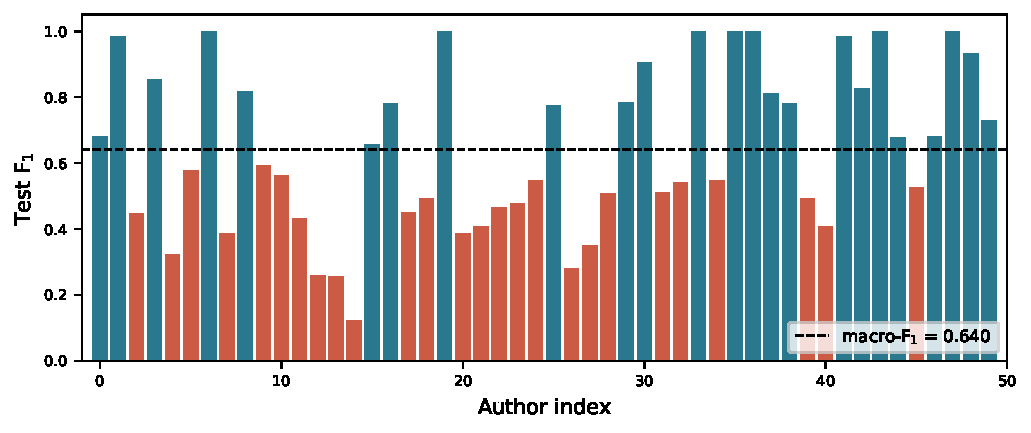
\includegraphics[width=\columnwidth]{figures/per_class_f1.pdf}
  \caption{Per-author test F$_1$ for the CNN-LSTM ensemble (50 authors). Bars below the dashed macro-F$_1$ line are highlighted; the long tail of low-F$_1$ authors drives the macro gap to the character $n$-gram baseline.}
  \label{fig:per-class-f1}
\end{figure}

\subsection{Confusion Analysis}

Figure~\ref{fig:confusion} shows the row-normalised CNN-LSTM test confusion matrix.
Off-diagonal mass concentrates on a handful of author pairs with similar post lengths and shared topical vocabulary, consistent with the weakest per-class scores above.

\begin{figure}[t]
  \centering
  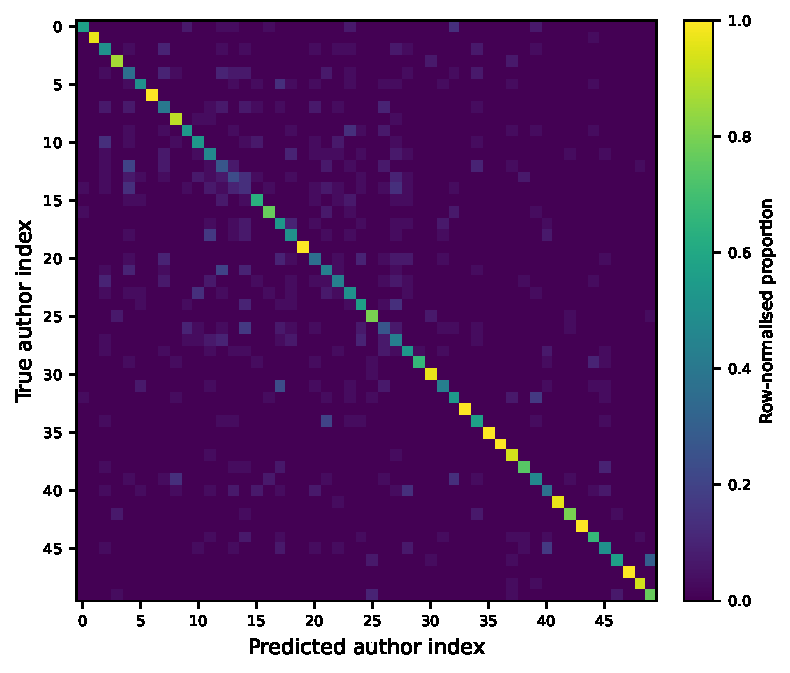
\includegraphics[width=0.86\columnwidth]{figures/confusion_matrix.pdf}
  \caption{Row-normalised confusion matrix for the CNN-LSTM ensemble on the held-out test split (50 authors). A bright diagonal indicates correct attribution; scattered off-diagonal cells mark systematic confusions.}
  \label{fig:confusion}
\end{figure}

\subsection{Training Dynamics}

Figure~\ref{fig:training-curves} traces the best individual ensemble member (seed 5): training loss falls steadily while validation macro-F$_1$ rises and plateaus, with the best checkpoint selected before early stopping.

\begin{figure}[t]
  \centering
  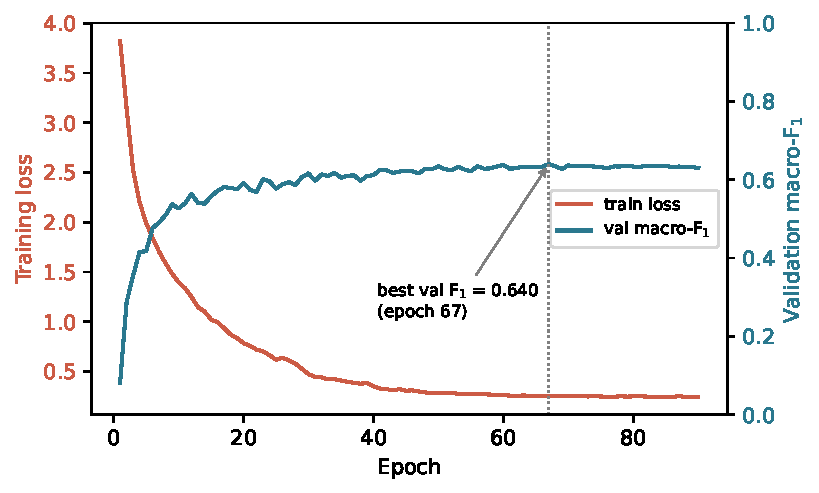
\includegraphics[width=\columnwidth]{figures/training_curves.pdf}
  \caption{CNN-LSTM training dynamics (seed 5): training loss and validation macro-F$_1$ vs.\ epoch, from the per-epoch trace in \texttt{training.json}.}
  \label{fig:training-curves}
\end{figure}

\section{Explainability and Error Analysis}
\label{sec:explainability}

\paragraph{SHAP.}
We apply KernelExplainer with 50 background samples, computing per-token attributions (\texttt{src/explainability.py}).
High-attribution tokens are predominantly punctuation patterns (repeated exclamation marks, ellipses), morphological fragments (\texttt{in} vs.\ \texttt{ing}, \texttt{ur} vs.\ \texttt{your}), and author-specific hashtag fragments: sub-lexical cues that BPE surfaces.

\paragraph{LIME (demonstrated).}
We run LIME (\(600\) perturbations) on the shipped ensemble checkpoint for individual test tweets via \texttt{ExplainabilityModule.explain\_lime}.
Figure~\ref{fig:lime} shows a representative case: a tweet correctly attributed to author~23 with probability \(\approx\!1.0\).
The strongest positive contributions are the \textbf{capitalised function words} ``I'', ``It'', ``On'', ``The'', ``Like'', and ``Really'', which reflect this author's habit of title-casing nearly every word, an orthographic style signal rather than topical content (content tokens such as ``CD'' and ``Faves'' contribute weakly or negatively).
This makes the model's decision \emph{inspectable}: the subword encoder keys on stylistic casing and function-word patterns, exactly the cues stylometry predicts.

\begin{figure}[t]
  \centering
  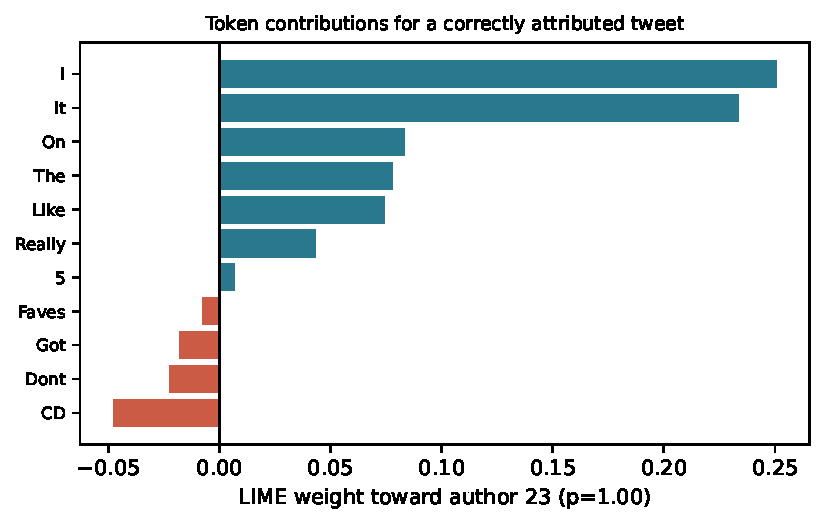
\includegraphics[width=\columnwidth]{figures/explainability_lime.pdf}
  \caption{LIME token contributions for a correctly attributed test tweet (author 23, \(p\!\approx\!1.0\)). Positive (blue) weights push toward the predicted author; the dominant cues are capitalised function words, evidence of a title-casing writing style.}
  \label{fig:lime}
\end{figure}

\paragraph{Misclassification analysis.}
Off-diagonal mass in the CNN-LSTM confusion matrix (Figure~\ref{fig:confusion}) concentrates on author pairs with similar post lengths and topical overlap.
Authors with perfect or near-perfect F$_1$ often exhibit distinctive casing, punctuation, or rare stable BPE pieces; confused pairs share abbreviations and hashtag habits, so subword features struggle when orthographic styles converge.

\paragraph{Robustness scope.}
Our evaluation is \emph{in-domain}: a single English Twitter slice under one stratified split.
We therefore do not claim cross-dialect or cross-platform robustness; the casing cue in Figure~\ref{fig:lime}, for instance, would not transfer to a normalised or lower-cased corpus.
A full robustness study (different platforms, dialects, or time periods) is left as future work, consistent with the \emph{domain lock-in} caveat noted in \S\ref{sec:dataset}.

\section{Conclusion and Discussion}
\label{sec:conclusion}

We compared a CNN-LSTM on BPE subword sequences against eight classical baselines for 50-author Twitter attribution.
The neural ensemble (63.8\% accuracy, 0.640 macro-F$_1$) is competitive but slightly below character $n$-grams + SVM (66.2\%, 0.657).
SHAP/LIME highlight morphological fragments and punctuation; errors cluster where authors' surface styles overlap.
<<<<<<< HEAD
Answering our questions directly: \textbf{(RQ1)} the subword CNN-LSTM does learn stable author representations, reaching 0.640 macro-F$_1$ across all 50 authors; \textbf{(RQ2)} under the shared stratified split it is competitive with, but does not beat, the strongest classical feature (character $n$-grams + SVM, 0.657); and \textbf{(RQ3)} correct decisions hinge on orthographic and morphological subword cues (casing, punctuation, stable BPE fragments), while systematic confusions concentrate among authors with overlapping post length and topical vocabulary.
=======
>>>>>>> 520ef946993df07b9ed58b417b0deb9cfc9e205a

\textbf{Limitations:} Single English Twitter slice; closed-set labels; SHAP cost limits large-scale explanation; moderate data per author (200 posts) favours sample-efficient sparse features.

\textbf{Future work:} Attention over subword time steps; multilingual corpora; hybrid subword + character $n$-gram inputs; larger author sets with few-shot evaluation.

\section*{Ethics Statement}

Social-media authorship tools must be used responsibly: attribution on public benchmarks does not authorise non-consensual deanonymisation of private accounts.

\FloatBarrier
\bibliography{custom}

\end{document}
